% Slide-optimized version of fig_pipeline_tse.tex.
% Wider page, single-line labels with inline greek symbols, tighter vertical
% spacing so it fits a 16:9 beamer slide without awkward whitespace.
% The columnar/PNAS version lives in fig_pipeline_tse.tex.
\documentclass{article}
\usepackage[paperwidth=13in,paperheight=5.2in,margin=0.18in]{geometry}
\usepackage{amsmath, amssymb}
\usepackage{xcolor}
\usepackage{tikz}
\usetikzlibrary{arrows.meta, positioning, fit, backgrounds, calc}
\pagestyle{empty}

\begin{document}
\begin{center}
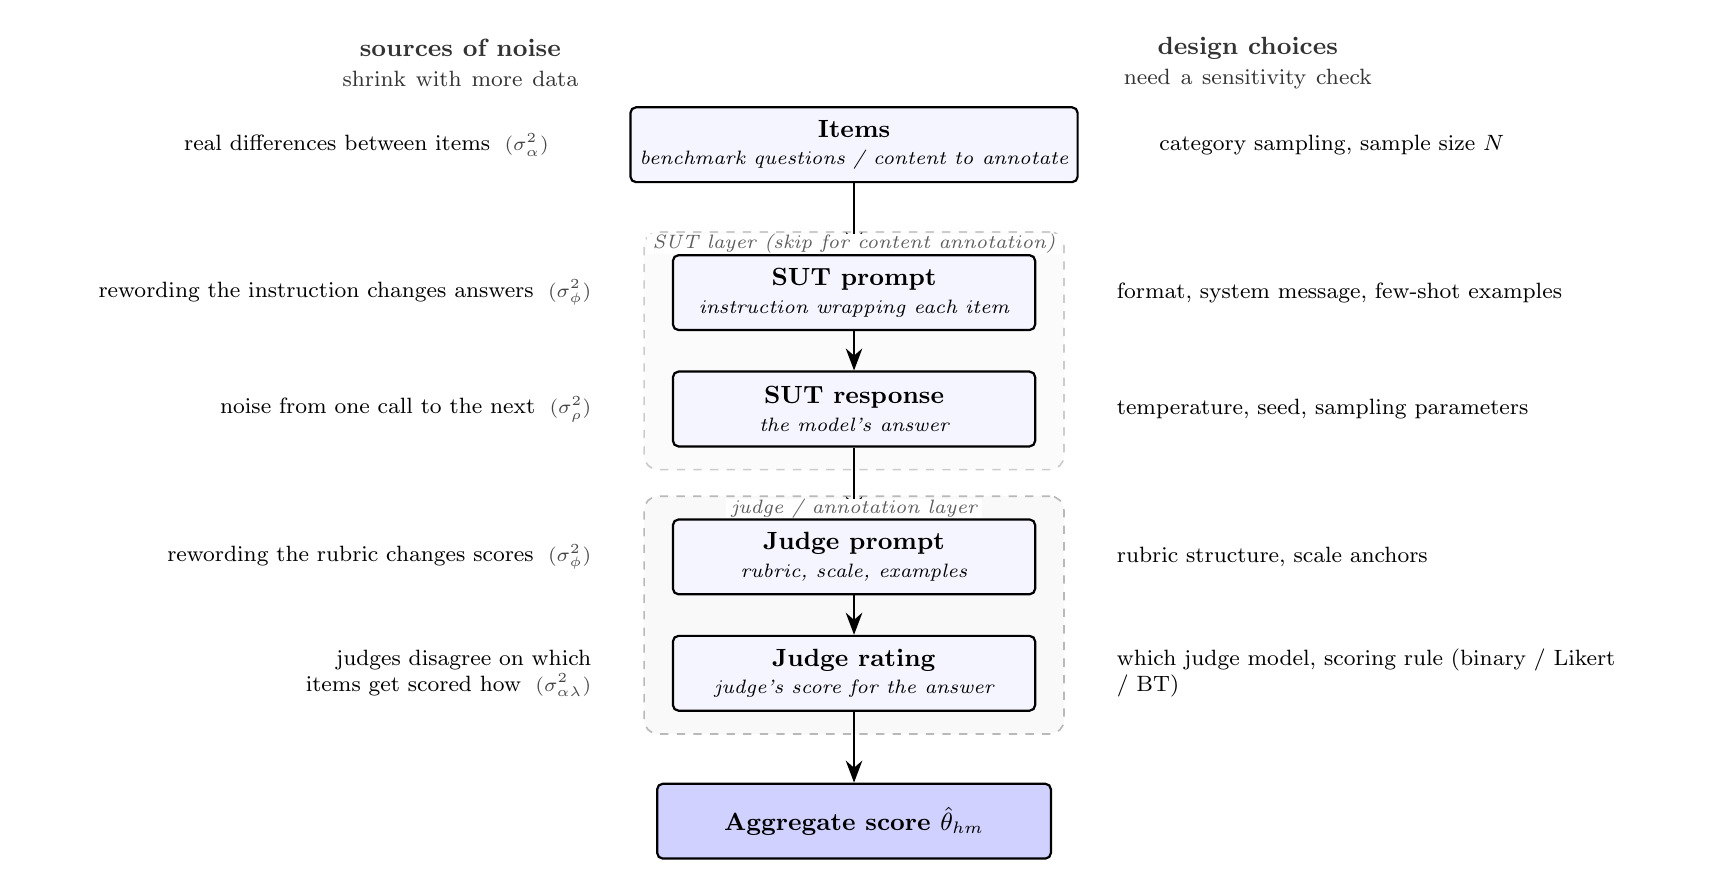
\begin{tikzpicture}[
    node distance=0.5cm and 2.2cm,
    box/.style    = {rectangle, draw, thick, rounded corners=2pt,
                     minimum width=4.6cm, minimum height=0.95cm,
                     align=center, font=\small, fill=blue!4},
    final/.style  = {box, fill=blue!18, font=\bfseries\small,
                     minimum width=5.0cm},
    layer/.style  = {draw=gray!55, dashed, semithick, rounded corners=5pt,
                     inner xsep=10pt, inner ysep=8pt, fill=gray!5},
    llabel/.style = {font=\scriptsize\itshape, text=gray!72!black,
                     fill=white, inner xsep=2pt, inner ysep=0pt},
    vleft/.style  = {font=\footnotesize, align=right, anchor=east,
                     text width=6.5cm},
    vright/.style = {font=\footnotesize, align=left,  anchor=west,
                     text width=6.5cm},
    arrow/.style  = {-{Stealth[length=2.8mm]}, thick},
    header/.style = {font=\small\bfseries, align=center,
                     text=gray!40!black, text width=6.5cm}
]

% ========= central pipeline =========
\node[box]                            (items)  {\textbf{Items}\\[-1pt]\scriptsize\itshape benchmark questions / content to annotate};
\node[box, below=0.9cm of items]      (sutpr)  {\textbf{SUT prompt}\\[-1pt]\scriptsize\itshape instruction wrapping each item};
\node[box, below=of sutpr]            (sutres) {\textbf{SUT response}\\[-1pt]\scriptsize\itshape the model's answer};
\node[box, below=0.9cm of sutres]     (jpr)    {\textbf{Judge prompt}\\[-1pt]\scriptsize\itshape rubric, scale, examples};
\node[box, below=of jpr]              (jres)   {\textbf{Judge rating}\\[-1pt]\scriptsize\itshape judge's score for the answer};
\node[final, below=0.9cm of jres]     (agg)    {Aggregate score $\hat{\theta}_{hm}$};

\draw[arrow] (items)  -- (sutpr);
\draw[arrow] (sutpr)  -- (sutres);
\draw[arrow] (sutres) -- (jpr);
\draw[arrow] (jpr)    -- (jres);
\draw[arrow] (jres)   -- (agg);

% ========= layer frames =========
\begin{scope}[on background layer]
  \node[layer, draw=gray!40, fill=gray!3,
        fit=(sutpr)(sutres)] (sutlayer) {};
  \node[layer, fit=(jpr)(jres)]      (jlayer)   {};
\end{scope}
\node[llabel, anchor=north] at ([yshift=-1pt]sutlayer.north)
   {SUT layer (skip for content annotation)};
\node[llabel, anchor=north] at ([yshift=-1pt]jlayer.north)
   {judge / annotation layer};

% ========= LEFT: random variance, inline symbols, one line each =========
\node[vleft] at ([xshift=-0.9cm]items.west)
    {real differences between items \;{\scriptsize\textcolor{gray!55!black}{$(\sigma^{2}_{\alpha})$}}};
\node[vleft] at ([xshift=-0.9cm]sutpr.west)
    {rewording the instruction changes answers \;{\scriptsize\textcolor{gray!55!black}{$(\sigma^{2}_{\phi})$}}};
\node[vleft] at ([xshift=-0.9cm]sutres.west)
    {noise from one call to the next \;{\scriptsize\textcolor{gray!55!black}{$(\sigma^{2}_{\rho})$}}};
\node[vleft] at ([xshift=-0.9cm]jpr.west)
    {rewording the rubric changes scores \;{\scriptsize\textcolor{gray!55!black}{$(\sigma^{2}_{\phi})$}}};
\node[vleft] at ([xshift=-0.9cm]jres.west)
    {judges disagree on which items get scored how \;{\scriptsize\textcolor{gray!55!black}{$(\sigma^{2}_{\alpha\lambda})$}}};

% ========= RIGHT: design choices, single line each =========
\node[vright] at ([xshift=0.9cm]items.east)
    {category sampling, sample size $N$};
\node[vright] at ([xshift=0.9cm]sutpr.east)
    {format, system message, few-shot examples};
\node[vright] at ([xshift=0.9cm]sutres.east)
    {temperature, seed, sampling parameters};
\node[vright] at ([xshift=0.9cm]jpr.east)
    {rubric structure, scale anchors};
\node[vright] at ([xshift=0.9cm]jres.east)
    {which judge model, scoring rule (binary / Likert / BT)};

% ========= column headers =========
\node[header] at ([xshift=-5.0cm,yshift=0.55cm]items.north)
    {sources of noise\\{\normalfont\footnotesize shrink with more data}};
\node[header] at ([xshift=5.0cm,yshift=0.55cm]items.north)
    {design choices\\{\normalfont\footnotesize need a sensitivity check}};

\end{tikzpicture}
\end{center}
\end{document}
